% Options for packages loaded elsewhere
\PassOptionsToPackage{unicode}{hyperref}
\PassOptionsToPackage{hyphens}{url}
%
\documentclass[
]{book}
\usepackage{amsmath,amssymb}
\usepackage{lmodern}
\usepackage{ifxetex,ifluatex}
\ifnum 0\ifxetex 1\fi\ifluatex 1\fi=0 % if pdftex
  \usepackage[T1]{fontenc}
  \usepackage[utf8]{inputenc}
  \usepackage{textcomp} % provide euro and other symbols
\else % if luatex or xetex
  \usepackage{unicode-math}
  \defaultfontfeatures{Scale=MatchLowercase}
  \defaultfontfeatures[\rmfamily]{Ligatures=TeX,Scale=1}
\fi
% Use upquote if available, for straight quotes in verbatim environments
\IfFileExists{upquote.sty}{\usepackage{upquote}}{}
\IfFileExists{microtype.sty}{% use microtype if available
  \usepackage[]{microtype}
  \UseMicrotypeSet[protrusion]{basicmath} % disable protrusion for tt fonts
}{}
\makeatletter
\@ifundefined{KOMAClassName}{% if non-KOMA class
  \IfFileExists{parskip.sty}{%
    \usepackage{parskip}
  }{% else
    \setlength{\parindent}{0pt}
    \setlength{\parskip}{6pt plus 2pt minus 1pt}}
}{% if KOMA class
  \KOMAoptions{parskip=half}}
\makeatother
\usepackage{xcolor}
\IfFileExists{xurl.sty}{\usepackage{xurl}}{} % add URL line breaks if available
\IfFileExists{bookmark.sty}{\usepackage{bookmark}}{\usepackage{hyperref}}
\hypersetup{
  pdftitle={Basic Statistical Methods for Public Health},
  pdfauthor={Guy Mizrachi},
  hidelinks,
  pdfcreator={LaTeX via pandoc}}
\urlstyle{same} % disable monospaced font for URLs
\usepackage{color}
\usepackage{fancyvrb}
\newcommand{\VerbBar}{|}
\newcommand{\VERB}{\Verb[commandchars=\\\{\}]}
\DefineVerbatimEnvironment{Highlighting}{Verbatim}{commandchars=\\\{\}}
% Add ',fontsize=\small' for more characters per line
\usepackage{framed}
\definecolor{shadecolor}{RGB}{248,248,248}
\newenvironment{Shaded}{\begin{snugshade}}{\end{snugshade}}
\newcommand{\AlertTok}[1]{\textcolor[rgb]{0.94,0.16,0.16}{#1}}
\newcommand{\AnnotationTok}[1]{\textcolor[rgb]{0.56,0.35,0.01}{\textbf{\textit{#1}}}}
\newcommand{\AttributeTok}[1]{\textcolor[rgb]{0.77,0.63,0.00}{#1}}
\newcommand{\BaseNTok}[1]{\textcolor[rgb]{0.00,0.00,0.81}{#1}}
\newcommand{\BuiltInTok}[1]{#1}
\newcommand{\CharTok}[1]{\textcolor[rgb]{0.31,0.60,0.02}{#1}}
\newcommand{\CommentTok}[1]{\textcolor[rgb]{0.56,0.35,0.01}{\textit{#1}}}
\newcommand{\CommentVarTok}[1]{\textcolor[rgb]{0.56,0.35,0.01}{\textbf{\textit{#1}}}}
\newcommand{\ConstantTok}[1]{\textcolor[rgb]{0.00,0.00,0.00}{#1}}
\newcommand{\ControlFlowTok}[1]{\textcolor[rgb]{0.13,0.29,0.53}{\textbf{#1}}}
\newcommand{\DataTypeTok}[1]{\textcolor[rgb]{0.13,0.29,0.53}{#1}}
\newcommand{\DecValTok}[1]{\textcolor[rgb]{0.00,0.00,0.81}{#1}}
\newcommand{\DocumentationTok}[1]{\textcolor[rgb]{0.56,0.35,0.01}{\textbf{\textit{#1}}}}
\newcommand{\ErrorTok}[1]{\textcolor[rgb]{0.64,0.00,0.00}{\textbf{#1}}}
\newcommand{\ExtensionTok}[1]{#1}
\newcommand{\FloatTok}[1]{\textcolor[rgb]{0.00,0.00,0.81}{#1}}
\newcommand{\FunctionTok}[1]{\textcolor[rgb]{0.00,0.00,0.00}{#1}}
\newcommand{\ImportTok}[1]{#1}
\newcommand{\InformationTok}[1]{\textcolor[rgb]{0.56,0.35,0.01}{\textbf{\textit{#1}}}}
\newcommand{\KeywordTok}[1]{\textcolor[rgb]{0.13,0.29,0.53}{\textbf{#1}}}
\newcommand{\NormalTok}[1]{#1}
\newcommand{\OperatorTok}[1]{\textcolor[rgb]{0.81,0.36,0.00}{\textbf{#1}}}
\newcommand{\OtherTok}[1]{\textcolor[rgb]{0.56,0.35,0.01}{#1}}
\newcommand{\PreprocessorTok}[1]{\textcolor[rgb]{0.56,0.35,0.01}{\textit{#1}}}
\newcommand{\RegionMarkerTok}[1]{#1}
\newcommand{\SpecialCharTok}[1]{\textcolor[rgb]{0.00,0.00,0.00}{#1}}
\newcommand{\SpecialStringTok}[1]{\textcolor[rgb]{0.31,0.60,0.02}{#1}}
\newcommand{\StringTok}[1]{\textcolor[rgb]{0.31,0.60,0.02}{#1}}
\newcommand{\VariableTok}[1]{\textcolor[rgb]{0.00,0.00,0.00}{#1}}
\newcommand{\VerbatimStringTok}[1]{\textcolor[rgb]{0.31,0.60,0.02}{#1}}
\newcommand{\WarningTok}[1]{\textcolor[rgb]{0.56,0.35,0.01}{\textbf{\textit{#1}}}}
\usepackage{longtable,booktabs,array}
\usepackage{calc} % for calculating minipage widths
% Correct order of tables after \paragraph or \subparagraph
\usepackage{etoolbox}
\makeatletter
\patchcmd\longtable{\par}{\if@noskipsec\mbox{}\fi\par}{}{}
\makeatother
% Allow footnotes in longtable head/foot
\IfFileExists{footnotehyper.sty}{\usepackage{footnotehyper}}{\usepackage{footnote}}
\makesavenoteenv{longtable}
\usepackage{graphicx}
\makeatletter
\def\maxwidth{\ifdim\Gin@nat@width>\linewidth\linewidth\else\Gin@nat@width\fi}
\def\maxheight{\ifdim\Gin@nat@height>\textheight\textheight\else\Gin@nat@height\fi}
\makeatother
% Scale images if necessary, so that they will not overflow the page
% margins by default, and it is still possible to overwrite the defaults
% using explicit options in \includegraphics[width, height, ...]{}
\setkeys{Gin}{width=\maxwidth,height=\maxheight,keepaspectratio}
% Set default figure placement to htbp
\makeatletter
\def\fps@figure{htbp}
\makeatother
\setlength{\emergencystretch}{3em} % prevent overfull lines
\providecommand{\tightlist}{%
  \setlength{\itemsep}{0pt}\setlength{\parskip}{0pt}}
\setcounter{secnumdepth}{5}
\ifluatex
  \usepackage{selnolig}  % disable illegal ligatures
\fi

\title{Basic Statistical Methods for Public Health}
\author{Guy Mizrachi}
\date{2021-10-20}

\begin{document}
\maketitle

{
\setcounter{tocdepth}{1}
\tableofcontents
}
\begin{Shaded}
\begin{Highlighting}[]
\NormalTok{bookdown}\SpecialCharTok{::}\FunctionTok{render\_book}\NormalTok{(}\AttributeTok{new\_session =} \ConstantTok{TRUE}\NormalTok{, }\AttributeTok{output\_format =} \StringTok{"HTML"}\NormalTok{)}
\end{Highlighting}
\end{Shaded}

\begin{Shaded}
\begin{Highlighting}[]
\NormalTok{bookdown}\SpecialCharTok{::}\FunctionTok{serve\_book}\NormalTok{()}
\end{Highlighting}
\end{Shaded}

\hypertarget{introduction}{%
\chapter{Introduction}\label{introduction}}

This is an R bookdown format, which will be used to show examples of answers to questions from the course's book.
Using this format is supposed to be intuitive, each `book' will contain chapters, each chapter is a question.

Using R bookdown will allow us to show the question's data and principles through both explanations and visualization.

\textbf{Good luck!}

Guy.

\hypertarget{set-a-question-1}{%
\chapter{Set A question 1}\label{set-a-question-1}}

(Page 20)

\hypertarget{question}{%
\section{Question}\label{question}}

``In the U.S In 2000, there were 2.4 million deaths from all causes, compared to 1.9 million in 1970 - a 25\% increase.
True or false, and explain: the data show that the public's health got worse over the period 1970-2000.''

\hypertarget{answer}{%
\section{Answer}\label{answer}}

\textbf{FALSE}

Explain: Although the data points towards an overall increase in deaths,
it fails to show weather the public's health got worse over that time period.

An absolute growth (from 1.9 million to 2.4 million) does not suggest \textbf{a relative growth}.
It is safe to assume that the population got bigger as well, which can explain the increase in
absolute number of deaths.

Let's look at an example of relative and absolute numbers (the population number is just for example):

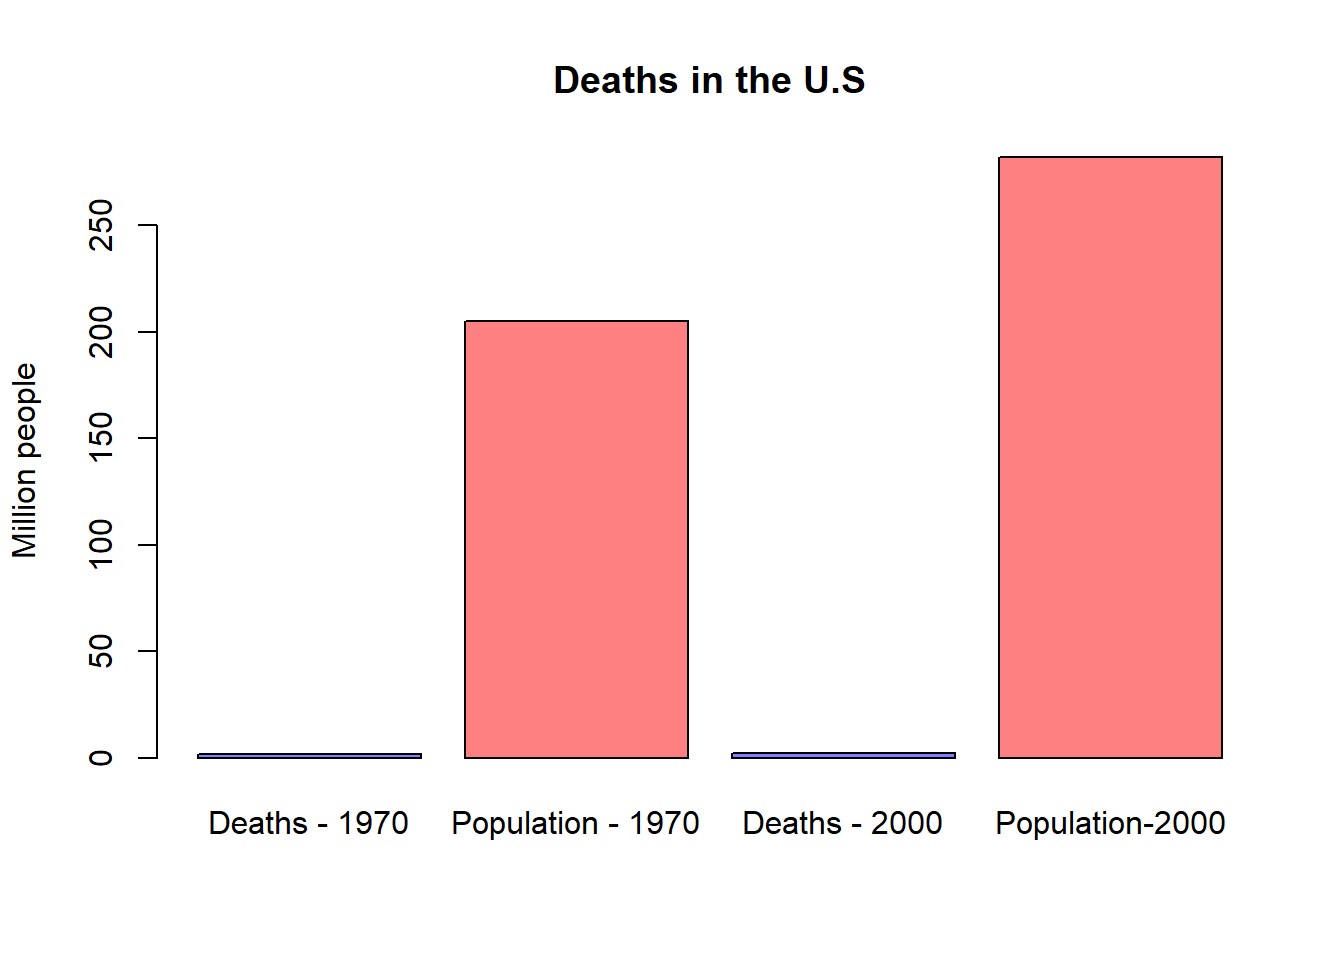
\includegraphics{_main_files/figure-latex/unnamed-chunk-4-1.pdf}

As we can see, although the absolute number of deaths shows an increase of 25\%, the relative deaths per population shows a decrease, which contradicts the conclusion that the public's health has got worse.

Let's look at the relative numbers:

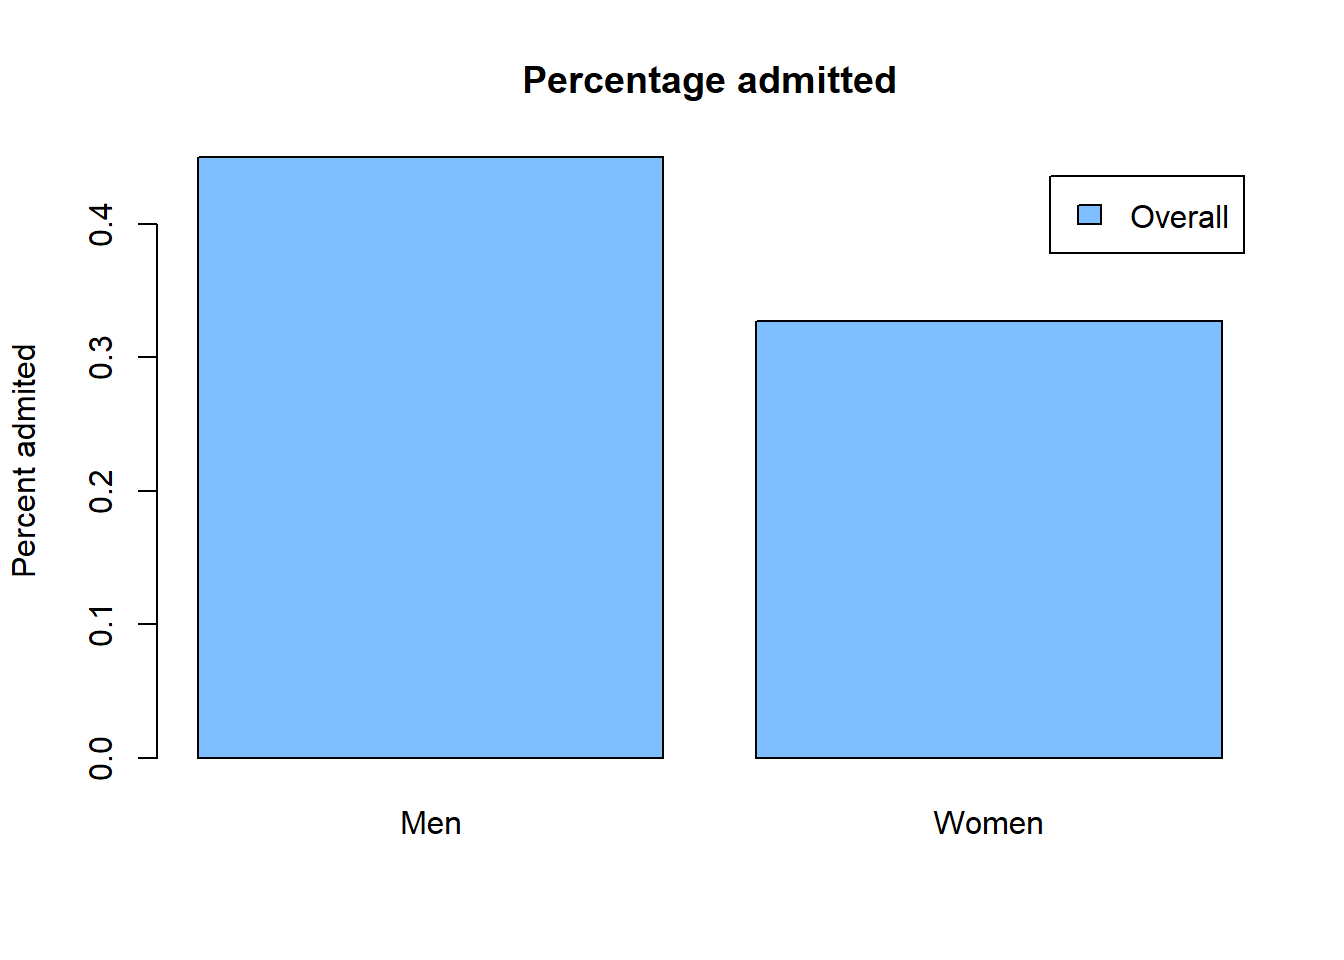
\includegraphics{_main_files/figure-latex/unnamed-chunk-5-1.pdf}

\hypertarget{set-a-question-3}{%
\chapter{Set A question 3}\label{set-a-question-3}}

(Page 21)

\hypertarget{question-1}{%
\section{Question}\label{question-1}}

``Polio is an infectious disease; for example, it seemed to spread when children went swimming together. The
NFIP study was not done blind: could that bias the results? Discuss briefly''

\hypertarget{answer-1}{%
\section{Answer}\label{answer-1}}

\textbf{Yes}, that could create a bias.
A study which was not done blind (meaning: the subjects were chosen, not randomly) could have a number of biases for/against the vaccine.
If we were to choose children that engage in activites (like swimming) that increased their chances of getting the virus, it would have been a bias against the vaccine.

\hypertarget{set-a-question-12}{%
\chapter{Set A Question 12}\label{set-a-question-12}}

(page 23)

\hypertarget{question-2}{%
\section{Question}\label{question-2}}

``Physical exercise is considered to increase the risk of spontaneous abortion. Furthermore, women who have had a spontaneous abortion are more likely to have another. One observational study finds that women who exercise regularly have fewer spontaneous abortions than other women. Can you explain the findings of this study?''

\hypertarget{answer-2}{%
\section{Answer}\label{answer-2}}

Women who exercise regularly may not have had any spontaneous abortion in the past, otherwise - they would not have continued to exercise regularly. This study can be explained by \textbf{the selection process} between those women: those who exercise regularly are in good health and did not experience spontaneous abortion until now.

\hypertarget{set-a-question-13}{%
\chapter{Set A question 13}\label{set-a-question-13}}

(Page 24)

\hypertarget{question-3}{%
\section{Question}\label{question-3}}

``A hypothetical university has two departments, A and B. There are 2,000 male applicants, of whom half apply to each department. There are 1,100 female applicants: 100 apply to department A and 1,000 to department B. Department A admits 60\% of the men who apply and 60\% of the women. Department B admits 30\% of the men who apply and 30\% of the women.' For each department, the percentage of men admitted equals the percentage of women admitted; this must be so for both departments together.' True or false, and explain briefly''

\hypertarget{answer-3}{%
\section{Answer}\label{answer-3}}

\textbf{FALSE}

Let's check how many men and women were admitted:

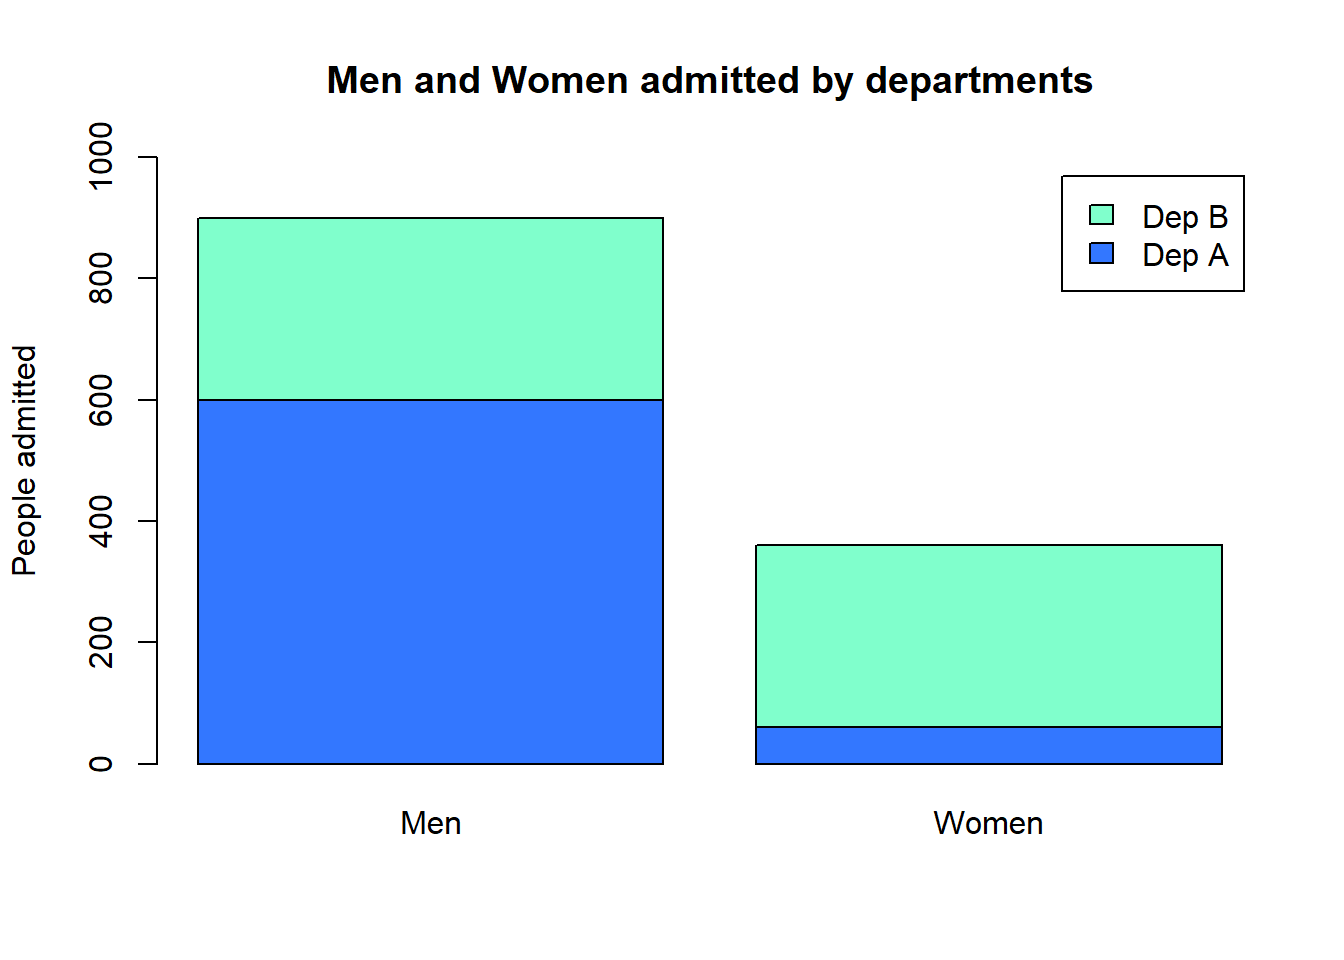
\includegraphics{_main_files/figure-latex/unnamed-chunk-6-1.pdf}

We can see that more men were admitted than women, but let's compare the admission percent (divide by number of men or women):

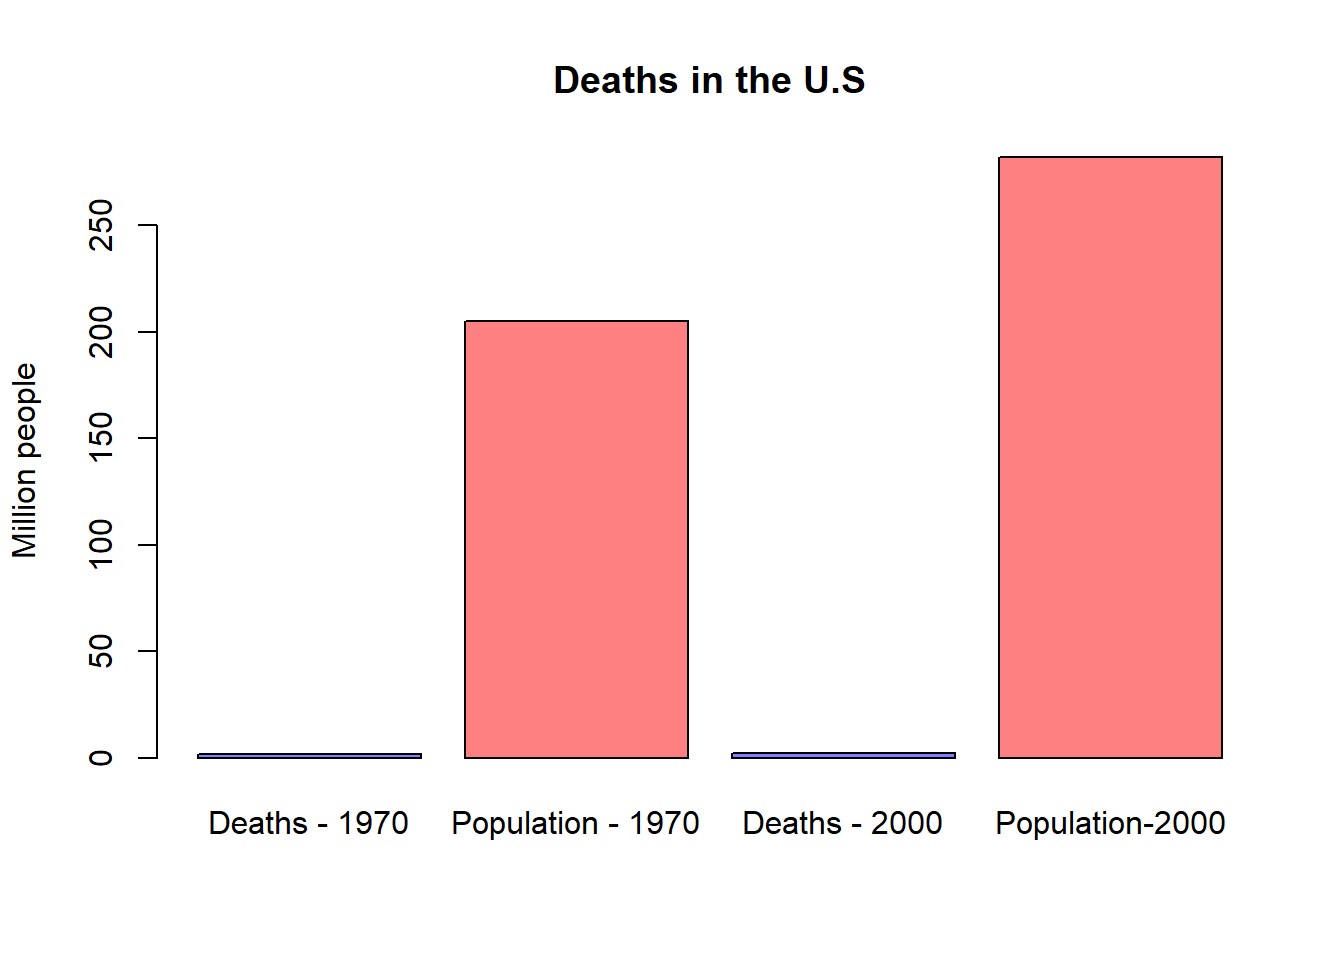
\includegraphics{_main_files/figure-latex/unnamed-chunk-7-1.pdf}

Although each department accepted the same percent, with no regard to men/women applicants, higher percentage of men were admitted due to the higher applications for department A (50\% of men) comparing to the women's. Department A's admission chances were higher (60\%) than department B's, so a higher percentage of men were admitted.

\end{document}
